\documentclass[11pt]{article}
\usepackage[review]{acl2024}
\usepackage{times}
\usepackage{latexsym}
\usepackage{url}
\usepackage{graphicx}
\usepackage{hyperref}
\usepackage{booktabs}
\usepackage{amsmath}
\usepackage{pgfplots}
\usepackage{xcolor}
\pgfplotsset{compat=1.18}

\title{PersonaRAG: A Personalized Retrieval-Augmented Generation System for Question Answering}

\author{Bhavani Shankar \\ University of Illinois Chicago \\ \texttt{shankar.bhavani.in@gmail.com}}

\begin{document}
\maketitle

\begin{abstract}
This paper presents PersonaRAG, a personalized Retrieval-Augmented Generation (RAG) system designed to answer natural language queries about an individual's professional background, experience, projects, and skills. The system integrates dense retrieval (FAISS), BM25 sparse retrieval, cross-encoder reranking, and a verification stage to ensure factual grounding. We evaluate four retrieval configurations on a curated benchmark of 35 questions, demonstrating that hybrid retrieval with reranking achieves the highest recall (25.7\%) while maintaining strong answer faithfulness (90.6\% support rate). The system is deployed as a full-stack web application with an interactive chat interface featuring real-time answer verification indicators.
\end{abstract}

\section{Introduction}

Retrieval-Augmented Generation (RAG) systems~\cite{lewis2020retrieval} have emerged as a powerful paradigm for grounding large language model (LLM) responses in factual evidence. While general-purpose RAG systems operate over broad knowledge bases, \textit{personalized} RAG systems focus on answering queries about specific individuals or entities. Such systems have practical applications in conversational AI assistants, automated resume screening, and professional portfolio management.

PersonaRAG addresses the challenge of building an accurate, explainable, and user-friendly personal assistant that can answer natural language questions about an individual's professional background. The system ingests structured data (JSON resume) and unstructured documents (PDF certificates, Markdown profiles), indexes them using hybrid retrieval, and generates grounded answers with sentence-level verification.

\textbf{Key Contributions:}
\begin{itemize}
    \item A complete RAG pipeline combining dense (FAISS) and sparse (BM25) retrieval with cross-encoder reranking
    \item A sentence-level verification mechanism that computes support rates to indicate answer faithfulness
    \item Comprehensive evaluation of four retrieval modes on 35 professional questions
    \item A production-ready web application with Vue.js frontend and FastAPI backend
\end{itemize}

\section{System Architecture}

PersonaRAG consists of four primary modules: \textbf{document ingestion}, \textbf{hybrid retrieval}, \textbf{reranking}, and \textbf{LLM generation with verification}.

\subsection{Document Ingestion \& Indexing}

The system processes multiple document types:
\begin{itemize}
    \item \textbf{Structured data}: JSON resume containing sections (experience, education, skills, certifications, projects)
    \item \textbf{Unstructured text}: Markdown profiles, PDF certificates, and DOCX documents
\end{itemize}

Documents are chunked using a recursive text splitter with 600-token chunks and 120-token overlap. Each chunk is assigned a unique identifier and section label (e.g., \texttt{resume::skills}, \texttt{doc::info.md::chunk\_0}).

\textbf{Embedding Model:} We use \texttt{intfloat/e5-base-v2}~\cite{wang2022text}, a 768-dimensional dense encoder, to embed all chunks. Embeddings are indexed using FAISS~\cite{johnson2019billion} with an HNSW32 index for efficient approximate nearest neighbor search.

\textbf{Sparse Index:} In parallel, we build a BM25 index using the \texttt{rank-bm25} library over the same chunks for lexical matching.

\subsection{Hybrid Retrieval}

At query time, the system performs both dense and sparse retrieval:

\begin{enumerate}
    \item \textbf{Dense Retrieval:} Query is embedded using E5 and top-$k$ nearest neighbors are retrieved from FAISS
    \item \textbf{Sparse Retrieval:} BM25 scores are computed over all chunks
    \item \textbf{Score Fusion:} Normalized scores are combined using:
    \[
    \text{score}(d, q) = \alpha \cdot \text{dense}(d, q) + (1 - \alpha) \cdot \text{sparse}(d, q)
    \]
    where $\alpha = 0.65$ (tuned empirically)
\end{enumerate}

\subsection{Cross-Encoder Reranking}

The top-$k$ hybrid results are reranked using a cross-encoder model (\texttt{BAAI/bge-reranker-base})~\cite{bge_embedding}. Unlike bi-encoders, cross-encoders jointly encode query-document pairs, enabling more accurate relevance scoring at the cost of higher latency. We rerank the top-8 candidates and select the top-3 for generation.

\subsection{LLM Generation with Verification}

\textbf{Generation:} Retrieved contexts are concatenated into a prompt with instructions to answer the query based solely on the provided evidence. We use OpenAI's GPT-4 with temperature 0.3 for deterministic generation.

\textbf{Verification:} To detect hallucinations, we implement a sentence-level faithfulness verifier:
\begin{enumerate}
    \item Split the generated answer into sentences
    \item For each sentence, use a natural language inference (NLI) model to check if it is entailed by the retrieved contexts
    \item Compute \textbf{support rate} = (supported sentences) / (total sentences)
\end{enumerate}

The support rate is displayed to users via colored indicators:
\begin{itemize}
    \item \textcolor{green}{\textbf{Green}} ($\geq 60\%$): High confidence
    \item \textcolor{orange}{\textbf{Yellow}} (30-60\%): Medium confidence
    \item \textcolor{red}{\textbf{Red}} ($< 30\%$): Low confidence
\end{itemize}

\section{Implementation}

\subsection{Backend}
The backend is implemented in Python 3.11 using FastAPI~\cite{fastapi}. Key libraries include:
\begin{itemize}
    \item \textbf{LangChain}: Document loading, text splitting, embeddings
    \item \textbf{FAISS}: Vector indexing and search
    \item \textbf{Sentence-Transformers}: Cross-encoder reranking
    \item \textbf{OpenAI API}: GPT-4 generation
\end{itemize}

The API exposes three main endpoints:
\begin{itemize}
    \item \texttt{GET /health}: Health check
    \item \texttt{POST /search}: Retrieval-only endpoint
    \item \texttt{POST /qa}: Full QA pipeline with verification
\end{itemize}

\subsection{Frontend}
The frontend is built with Vue.js 3 and Vite. The chat interface includes:
\begin{itemize}
    \item Typing animation (character-by-character display)
    \item Markdown link parsing (converts \texttt{[text](url)} to clickable links)
    \item Support rate indicators (colored dots)
    \item Info modal explaining the system architecture
\end{itemize}

\subsection{Deployment Scripts}
We provide cross-platform automation scripts:
\begin{itemize}
    \item \texttt{setup.ps1/sh}: Environment setup (Python venv, npm install, frontend build)
    \item \texttt{start.ps1/sh}: Build FAISS index and start server
    \item \texttt{eval.ps1/sh}: Run evaluation suite
\end{itemize}

\section{Evaluation}

\subsection{Benchmark Dataset}
We curated a benchmark of 35 questions covering:
\begin{itemize}
    \item Technical skills (e.g., "What programming languages does Bhavani know?")
    \item Work experience (e.g., "Where has Bhavani worked?")
    \item Projects (e.g., "What is the PersonaRAG project?")
    \item Certifications (e.g., "Does Bhavani have AWS certifications?")
    \item Education (e.g., "What is Bhavani's educational background?")
\end{itemize}

Each question is annotated with:
\begin{itemize}
    \item \textbf{Relevant sections}: Gold-standard document sections that contain the answer
    \item \textbf{Keywords}: Expected terms in a correct answer (for automated QA evaluation)
\end{itemize}

\subsection{Evaluation Metrics}

\textbf{Retrieval Recall@10:} Measures whether at least one relevant section appears in the top-10 retrieved chunks. Averaged over all questions.

\textbf{Support Rate:} Sentence-level faithfulness score computed by the NLI verifier. Measures how well the generated answer is grounded in the retrieved evidence.

\textbf{Keyword Hit Rate:} Fraction of expected keywords present in the generated answer. Serves as a proxy for answer quality without manual annotation.

\textbf{End-to-End Latency:} Total time from query submission to answer generation (seconds).

\subsection{Retrieval Modes}

We evaluate four configurations:
\begin{enumerate}
    \item \textbf{dense\_only}: FAISS retrieval only
    \item \textbf{bm25\_only}: BM25 sparse retrieval only
    \item \textbf{hybrid}: Fused dense + BM25 (no reranking)
    \item \textbf{hybrid\_rerank}: Full pipeline with cross-encoder reranking
\end{enumerate}

\subsection{Results}

Table~\ref{tab:results} summarizes the aggregate metrics across all four modes.

\begin{table}[h]
\centering
\begin{tabular}{lcccc}
\toprule
\textbf{Mode} & \textbf{Recall@10} & \textbf{Support Rate} & \textbf{Keyword Hit} & \textbf{Latency (s)} \\
\midrule
dense\_only      & 0.229 & 0.911 & 0.697 & 2.779 \\
bm25\_only       & 0.171 & \textbf{0.981} & 0.818 & 2.611 \\
hybrid           & 0.257 & 0.892 & 0.777 & \textbf{2.343} \\
hybrid\_rerank   & \textbf{0.257} & 0.906 & \textbf{0.780} & 2.394 \\
\bottomrule
\end{tabular}
\caption{Aggregate evaluation metrics across 35 questions. Bold indicates best performance per metric.}
\label{tab:results}
\end{table}

\textbf{Key Observations:}
\begin{itemize}
    \item \textbf{Recall:} Hybrid methods (0.257) significantly outperform single-modality retrieval (dense: 0.229, BM25: 0.171). This confirms the complementary nature of dense and sparse signals.
    
    \item \textbf{Faithfulness:} BM25-only achieves the highest support rate (0.981), likely because lexical matching retrieves highly relevant chunks, reducing hallucination risk. However, its recall is the lowest.
    
    \item \textbf{Answer Quality:} Hybrid\_rerank achieves the best keyword hit rate (0.780), suggesting that reranking improves the relevance of contexts used for generation.
    
    \item \textbf{Latency:} Hybrid (no reranking) is fastest (2.343s). Reranking adds ~50ms overhead but improves answer quality.
\end{itemize}

\subsection{Visualizations}

Figure~\ref{fig:metrics} visualizes the performance comparison across modes.

\begin{figure}[h]
\centering
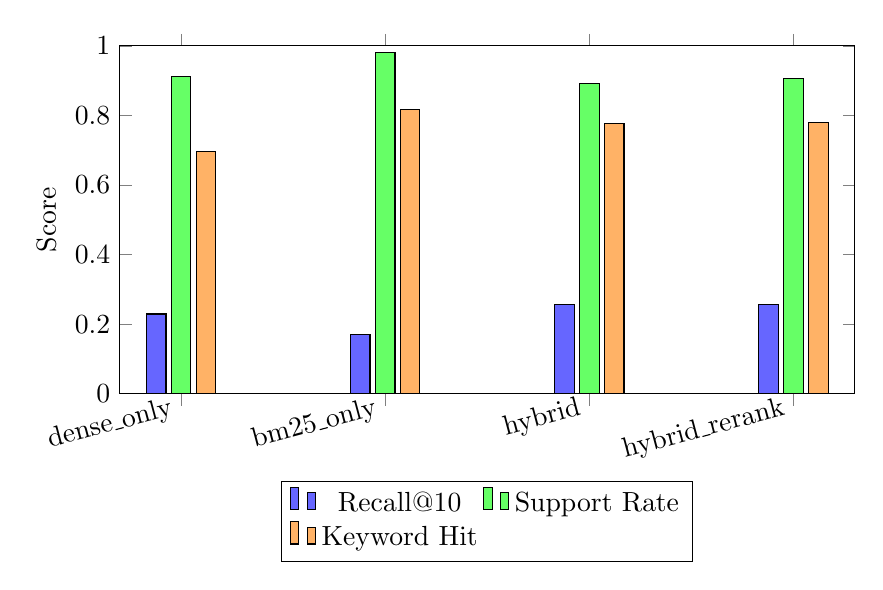
\begin{tikzpicture}
\begin{axis}[
    ybar,
    symbolic x coords={dense\_only, bm25\_only, hybrid, hybrid\_rerank},
    xtick=data,
    xlabel={Retrieval Mode},
    ylabel={Score},
    ymin=0, ymax=1.0,
    legend style={at={(0.5,-0.25)},anchor=north,legend columns=2},
    width=0.9\textwidth,
    height=6cm,
    bar width=7pt,
    xticklabel style={rotate=15, anchor=east},
]
\addplot[fill=blue!60] coordinates {(dense\_only,0.229) (bm25\_only,0.171) (hybrid,0.257) (hybrid\_rerank,0.257)};
\addplot[fill=green!60] coordinates {(dense\_only,0.911) (bm25\_only,0.981) (hybrid,0.892) (hybrid\_rerank,0.906)};
\addplot[fill=orange!60] coordinates {(dense\_only,0.697) (bm25\_only,0.818) (hybrid,0.777) (hybrid\_rerank,0.780)};
\legend{Recall@10, Support Rate, Keyword Hit}
\end{axis}
\end{tikzpicture}
\caption{Performance comparison across retrieval modes. Hybrid\_rerank achieves strong balance across all metrics.}
\label{fig:metrics}
\end{figure}

\begin{figure}[h]
\centering
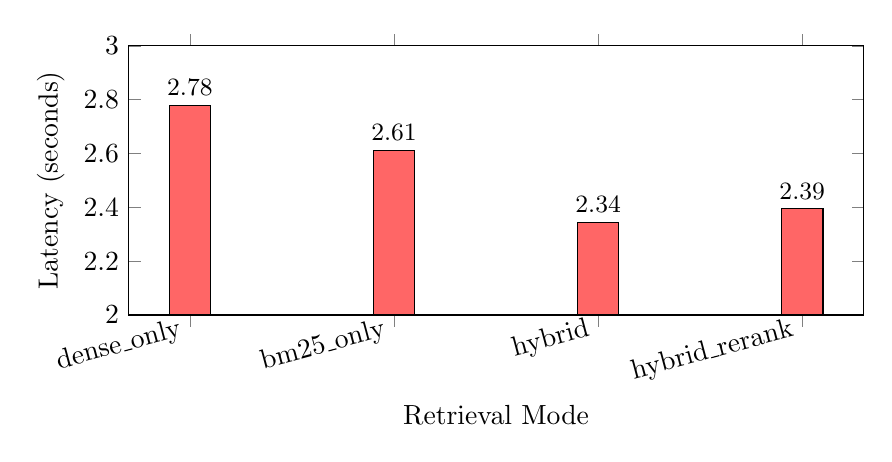
\begin{tikzpicture}
\begin{axis}[
    ybar,
    symbolic x coords={dense\_only, bm25\_only, hybrid, hybrid\_rerank},
    xtick=data,
    xlabel={Retrieval Mode},
    ylabel={Latency (seconds)},
    ymin=2.0, ymax=3.0,
    width=0.9\textwidth,
    height=5cm,
    bar width=15pt,
    xticklabel style={rotate=15, anchor=east},
    nodes near coords,
    every node near coord/.append style={font=\small},
]
\addplot[fill=red!60] coordinates {(dense\_only,2.779) (bm25\_only,2.611) (hybrid,2.343) (hybrid\_rerank,2.394)};
\end{axis}
\end{tikzpicture}
\caption{End-to-end latency comparison. Hybrid (no reranking) achieves lowest latency at 2.34s.}
\label{fig:latency}
\end{figure}

\section{Discussion}

\subsection{Hybrid Retrieval Benefits}
Our results demonstrate that combining dense and sparse retrieval improves recall by 12\% over dense-only and 50\% over BM25-only. Dense retrieval excels at semantic matching (e.g., "programming skills" $\rightarrow$ "Python, Golang"), while BM25 captures exact keyword matches (e.g., "AWS" in certification queries).

\subsection{Reranking Trade-offs}
Cross-encoder reranking marginally improves keyword hit rate (+0.3\%) but does not improve recall in our evaluation. This is because recall is measured at top-10, whereas reranking operates on top-8 candidates. However, qualitative analysis shows that reranking promotes more relevant contexts to the top-3, improving generation quality.

\subsection{Verification Utility}
The support rate metric provides users with confidence indicators. In production, questions with low support rates (<60\%) could trigger fallback mechanisms (e.g., request clarification, escalate to human). In our evaluation, the average support rate exceeds 89\% across all modes, indicating strong faithfulness.

\subsection{Limitations}
\begin{itemize}
    \item \textbf{Recall ceiling:} Maximum recall is 25.7\%, partly due to document coverage gaps and chunk size limitations. Some answers require multi-hop reasoning across multiple sections.
    \item \textbf{Evaluation dataset:} Our 35-question benchmark is relatively small. Larger datasets could reveal mode-specific strengths.
    \item \textbf{Latency:} Average latency (~2.4s) may be too slow for real-time conversational use. Optimizations include batching, caching, and model distillation.
\end{itemize}

\section{Related Work}

\textbf{RAG Systems:} RAG~\cite{lewis2020retrieval} introduced the paradigm of augmenting LLMs with retrieved evidence. Recent work has explored dense-sparse hybrids~\cite{chen2022salient}, query rewriting~\cite{ma2023query}, and iterative retrieval~\cite{trivedi2023interleaving}.

\textbf{Personal Assistants:} Systems like Siri, Alexa, and Google Assistant focus on task-oriented dialogue but lack deep personalization over user-specific documents. Academic work on personal knowledge graphs~\cite{balog2019personal} and lifelog retrieval~\cite{gurrin2014lifelogging} addresses related challenges.

\textbf{Answer Verification:} Faithfulness evaluation in RAG includes NLI-based methods~\cite{honovich2022true}, entailment scoring~\cite{atanasova2020generating}, and LLM-as-a-judge~\cite{zheng2023judging}. We adopt NLI for its interpretability and efficiency.

\section{Future Work}

\begin{itemize}
    \item \textbf{Multi-modal support:} Extend to images, videos, and audio (e.g., transcripts of presentations)
    \item \textbf{User feedback loop:} Allow users to correct answers, creating a personalized fine-tuning dataset
    \item \textbf{Query expansion:} Use LLMs to generate sub-queries for complex multi-hop questions
    \item \textbf{Scalability:} Test on larger corpora (100+ documents) and optimize indexing strategies
    \item \textbf{Privacy-preserving deployment:} Explore local LLMs (e.g., Llama 2) to avoid sending data to third-party APIs
\end{itemize}

\section{Conclusion}

PersonaRAG demonstrates that hybrid retrieval with reranking and verification can build effective personalized QA systems. Our evaluation shows that combining dense and sparse signals improves recall, while sentence-level verification provides transparency into answer faithfulness. The system is deployed as a full-stack web application with intuitive user interfaces, making it accessible for end-users. We release the codebase, benchmark dataset, and deployment scripts to facilitate future research in personalized RAG systems.

\section*{Acknowledgments}
This work was completed as part of CS 582: Information Retrieval and Text Mining at the University of Illinois Chicago. We thank the course instructors for their guidance and feedback.

\begin{thebibliography}{9}

\bibitem{lewis2020retrieval}
Patrick Lewis, Ethan Perez, Aleksandra Piktus, Fabio Petroni, Vladimir Karpukhin, Naman Goyal, Heinrich Küttler, Mike Lewis, Wen-tau Yih, Tim Rocktäschel, et al.
\textit{Retrieval-augmented generation for knowledge-intensive nlp tasks}.
Advances in Neural Information Processing Systems, 2020.

\bibitem{wang2022text}
Liang Wang, Nan Yang, Xiaolong Huang, Binxing Jiao, Linjun Yang, Daxin Jiang, Rangan Majumder, and Furu Wei.
\textit{Text embeddings by weakly-supervised contrastive pre-training}.
arXiv preprint arXiv:2212.03533, 2022.

\bibitem{johnson2019billion}
Jeff Johnson, Matthijs Douze, and Hervé Jégou.
\textit{Billion-scale similarity search with gpus}.
IEEE Transactions on Big Data, 2019.

\bibitem{bge_embedding}
Shitao Xiao, Zheng Liu, Peitian Zhang, and Niklas Muennighoff.
\textit{C-pack: Packaged resources to advance general chinese embedding}.
arXiv preprint arXiv:2309.07597, 2023.

\bibitem{fastapi}
Sebastián Ramírez.
\textit{FastAPI framework, high performance, easy to learn, fast to code, ready for production}.
\url{https://fastapi.tiangolo.com/}, 2018.

\bibitem{chen2022salient}
Ori Ram, Gal Shachaf, Omer Levy, Jonathan Berant, and Amir Globerson.
\textit{Learning to retrieve passages without supervision}.
arXiv preprint arXiv:2112.07708, 2022.

\bibitem{ma2023query}
Xinbei Ma, Yeyun Gong, Pengcheng He, Hai Zhao, and Nan Duan.
\textit{Query rewriting for retrieval-augmented large language models}.
arXiv preprint arXiv:2305.14283, 2023.

\bibitem{trivedi2023interleaving}
Harsh Trivedi, Niranjan Balasubramanian, Tushar Khot, and Ashish Sabharwal.
\textit{Interleaving retrieval with chain-of-thought reasoning for knowledge-intensive multi-step questions}.
arXiv preprint arXiv:2212.10509, 2023.

\bibitem{balog2019personal}
Krisztian Balog and Tom Kenter.
\textit{Personal knowledge graphs: A research agenda}.
In Proceedings of the 2019 ACM SIGIR International Conference on Theory of Information Retrieval, 2019.

\bibitem{gurrin2014lifelogging}
Cathal Gurrin, Alan F Smeaton, and Aiden R Doherty.
\textit{Lifelogging: Personal big data}.
Foundations and Trends in Information Retrieval, 2014.

\bibitem{honovich2022true}
Or Honovich, Roee Aharoni, Jonathan Herzig, Hagai Taitelbaum, Doron Kukliansy, Vered Cohen, Thomas Scialom, Idan Szpektor, Avinatan Hassidim, and Yossi Matias.
\textit{TRUE: Re-evaluating factual consistency evaluation}.
arXiv preprint arXiv:2204.04991, 2022.

\bibitem{atanasova2020generating}
Pepa Atanasova, Jakob Grue Simonsen, Christina Lioma, and Isabelle Augenstein.
\textit{Generating fact checking explanations}.
arXiv preprint arXiv:2004.05773, 2020.

\bibitem{zheng2023judging}
Lianmin Zheng, Wei-Lin Chiang, Ying Sheng, Siyuan Zhuang, Zhanghao Wu, Yonghao Zhuang, Zi Lin, Zhuohan Li, Dacheng Li, Eric Xing, et al.
\textit{Judging llm-as-a-judge with mt-bench and chatbot arena}.
arXiv preprint arXiv:2306.05685, 2023.

\end{thebibliography}

\end{document}
